\documentclass[8pt,xcolor = table, t]{beamer}

% For more theme options, https://deic.uab.cat/~iblanes/beamer_gallery/
\usetheme{Antibes}
% \usetheme{Berlin}
% \usetheme{default}
% \usetheme{Warsaw}
% \usetheme{AnnArbor}

\setbeamertemplate{navigation symbols}{}

\setbeamercovered{transparent}

% \definecolor{beamer@blendedblue}{rgb}{0.58,0,0.83}
\definecolor{beamer@blendedblue}{rgb}{0.4,0,0.5}
\setbeamercolor{structure}{fg=beamer@blendedblue}


\setbeamerfont{caption}{series=\normalfont,size=\fontsize{8}{8}} 


\usepackage{amsmath,amssymb,amsfonts,amsthm}
\usepackage{graphicx}
\usepackage{subcaption}

\usepackage{algorithm}
\usepackage{algpseudocode}
\usepackage{ragged2e}

% \definecolor{LightViolet}{RGB}{230,220,255}
% \setbeamercolor{frametitle}{bg=LightViolet}

% For table
\usepackage{multirow}
\usepackage{makecell}
\usepackage{multicol}
\usepackage{fancyhdr}
\usepackage{arydshln}
% \usepackage[table,xcdraw]{xcolor} % Unlike 'report', this won't work in 'beamer'

\newtheorem{proposition}{\textit{Proposition}}
\newtheorem{remark}{\textit{Remark}}

% \usepackage{biblatex}

\usepackage[style=ieee,citetracker=true]{biblatex}
\addbibresource{References.bib}
\renewcommand{\bibfont}{\normalfont\footnotesize}
% \appto\bibfont{\itshape}
\setbeamercolor{bibliography entry note}{fg=blue}
\setbeamercolor{bibliography entry author}{fg=blue}

\renewcommand{\familydefault}{\rmdefault}   % For Times New Roman font

% For justified texts in each slide
\renewcommand{\raggedright}{\leftskip=0pt \rightskip=0pt plus 0cm}

% \setbeamercovered{transparent}
\setbeamertemplate{caption}[numbered]

\settowidth{\leftmargini}{\usebeamertemplate{itemize item}}
\addtolength{\leftmargini}{\labelsep}

% \setbeamerfont{caption}{size=\scriptsize}

\usepackage{bm} 

\newcommand\unfootnote[1]{%
  \begingroup
  \renewcommand\thefootnote{}\footnote{#1}%
  \addtocounter{footnote}{-1}%
  \endgroup
}

\setbeamertemplate{footline}
{
  \leavevmode%
  \hbox{
  \begin{beamercolorbox}[wd=0.66\paperwidth,ht=2.25ex,dp=1ex,left]{institute in head/foot}%
    \usebeamerfont{institute in head/foot}{Department of Engineering, Durham University}\hspace*{1ex} 
  \end{beamercolorbox}
  \begin{beamercolorbox}[wd=0.33\paperwidth,ht=2.25ex,dp=1ex,right]{date in head/foot}%
    \usebeamerfont{date in head/foot}\insertshortdate{\today}\hspace*{2em}
    \insertframenumber{} / \inserttotalframenumber\hspace*{2ex} 
  \end{beamercolorbox}}
  \vskip0pt
}

% \logo{\includegraphics[scale=0.01]{IITKGP Logo.png}}

\title[DIRECT]{Decentralised Integration of Renewable Energy Sources Through Smart Grid Technologies  \texorpdfstring{\\}{} (DIRECT)}
%%%%%%%%%%%%%%%%%%%%%%%%% Author Style 1 %%%%%%%%%%%%%%%%%%%%%%%%%

\institute{
\includegraphics[height=1.50cm]{Figures/DU Logo.png}}
% \institute{
\includegraphics[height=1.50cm]{ReNU.png}}
\author{\texorpdfstring{\\}{} \textbf{Presenter: Alexis Aguilar}}

                      
% \institute{\includegraphics[height=1.50cm]{IITKGP Logo.png} \\ Department of Electrical Engineering \texorpdfstring{\\}{} INDIAN INSTITUTE OF TECHNOLOGY KHARAGPUR \texorpdfstring{\\}{} }

% \institute{
\includegraphics[height=1.00cm]{DU Logo.png}}

\date{}

\begin{document}
%%%%%%%%%%%%%%%%%%%%%%%%%%%%%%%%%%%%%%%%%%%%%%%%%%%%%%%%%%%%
\begin{frame}
    \maketitle
\end{frame}
%%%%%%%%%%%%%%%%%%%%%%%%%%%%%%%%%%%%%%%%%%%%%%%%%%%%%%%%%%%%
% \begin{frame}{Table of Contents}
%     \tableofcontents
% \end{frame}
%%%%%%%%%%%%%%%%%%%%%%%%%%%%%%%%%%%%%%%%%%%%%%%%%%%%%%%%%%%%

% \input{20240131}
\section{Introduction}

\begin{frame}[c]{}

\begin{itemize}
        \item<only@1>[] 
            \begin{figure}
                \centering
                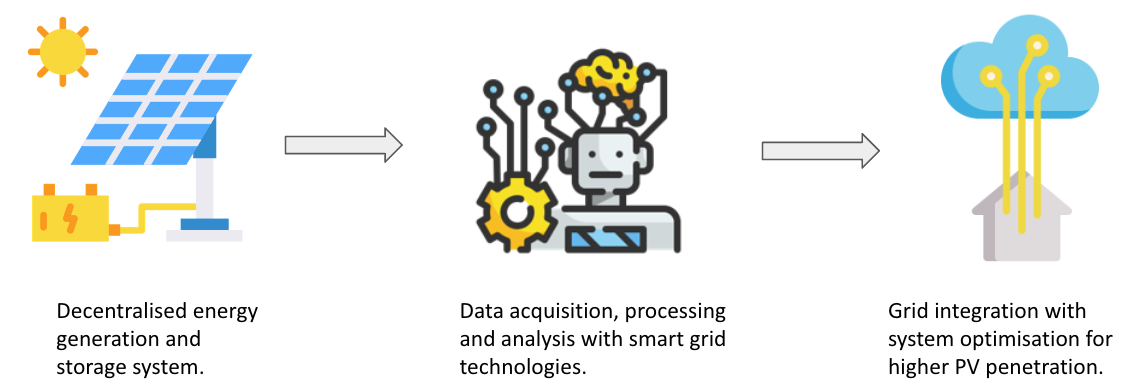
\includegraphics[width=1\linewidth]{Figures/DIRECT_Project.png}
                \caption{Fundamental areas of DIRECT Project.}
            \end{figure}

        \item<only@2>[]
            \begin{figure}
                \centering
                \begin{minipage}{0.6\linewidth}
                    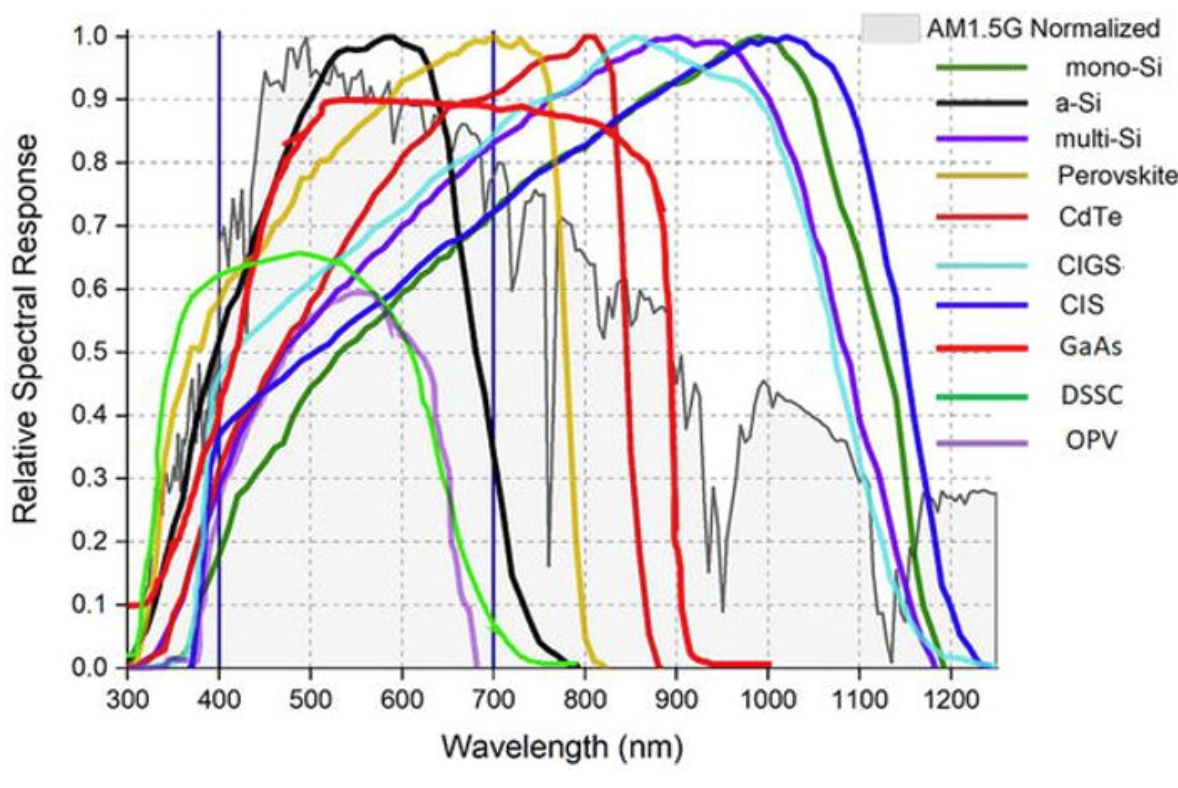
\includegraphics[width=\linewidth]{Figures/Material_response.png}
                    \caption{Spectral response per material}
                \end{minipage}%
                \begin{minipage}{0.4\linewidth}
                    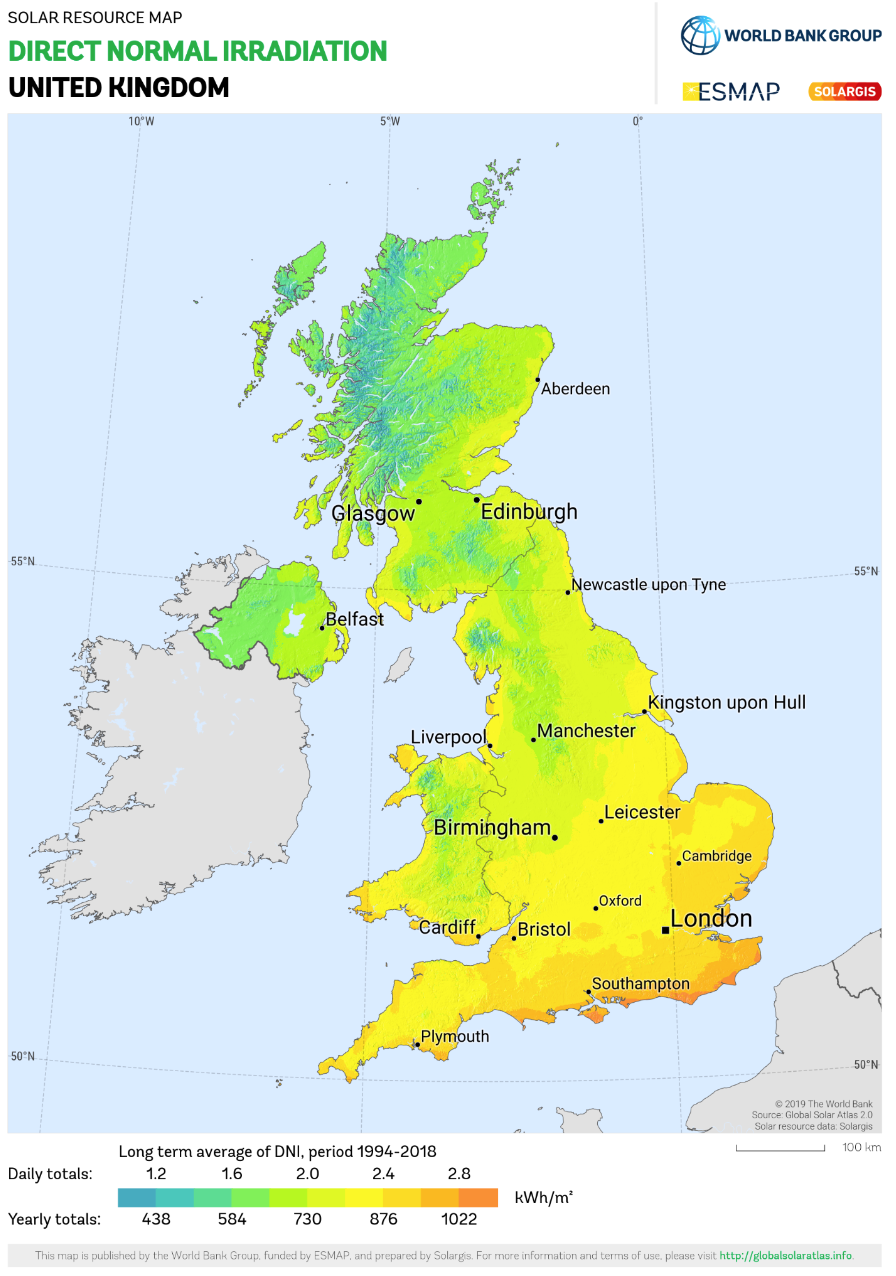
\includegraphics[width=\linewidth]{Figures/Irradiance distribution.png}
                    \caption{Annual irradiance distribution in the United Kingdom}
                \end{minipage}
            \end{figure} 
    \end{itemize}
\end{frame}

\section{PV and Self-Consumption Models}

\begin{frame}[c]{PV Single Diode Modeling}

    \begin{itemize}
        \item The Single Diode method defines the I-V (current-voltage) curve for a single-cell P-N junction as:\footnotemark[1] 
        \begin{subequations}
            \label{E:Solar_Power}
                \begin{equation} \label{eq1}
                    I=I_L-I_o({e^{\frac{q(V+IR_s)}{nkV_{th}}}-1})-{\frac{V+IR_s}{R_{sh}}}
                \end{equation}
        where \(I_L\) is the light current generated by the solar cell, \(I_o\) the diode reverse saturation current, 
        \(R_s\) series resistance, \(R_{sh}\) shunt resistance. \(N_s\) is the number of series-connected cells, \(q\) electron charge, \(k\) Boltzmann's constant, \(n\)
        is the ideality factor and \(T_c\) is the cell temperature.

        \item \(I_L\) can be calculated as:
                \begin{align}
                        I_L=\frac{S}{S_{ref}}(I_{L,ref}+\alpha_{I_{sc}}(T_c - T_{c,ref}))
                \end{align}
            \end{subequations} 
    \end{itemize}

    \footnotetext[1]{\fullcite{de2006improvement}}
\end{frame}

\begin{frame}[c]{PV Power Output from Single Diode Method}

    \begin{itemize}
        \item<only@{1}>        For any given traditional Silicon PV parameters evaluted with Eq. \ref{eq1}, the maximum power output would be calculated as:
        \begin{equation}\label{eq3}
            P_{SI-PV}^t(S,T_c) = V_{mpp}(S,T_c)I_{mpp}(S,T_c)
        \end{equation}
        where \(V_{mpp}\), \(I_{mpp}\) are the calculated voltage and current maximum power points in the I-V curve respectively for \(S\) and \(T_c\) at given time \(t\).

        \item<only@2> \textbf{Low-Light Enghanced PV} 
            Low-Light Enhanced PV (LLE-PV) output power is calculated based on Si-PV power output using Eq. \ref{eq3}. The power output of LLE-PV is determined as:
            
            \begin{equation}\label{eq4}
                P_{LLE-PV}^t(S,T_c) = P_{SI-PV}^t(S,T_c) \cdot \delta_{mat}(S,T_c)
            \end{equation}
            where \(\delta_{mat}\) is the potential PCE increase and decrease from irradiance and temperature based on the material characteristics.

        \item<only@3> \textbf{Calculating \(\delta_{mat}\):}

            This coefficient is determined by the expected temperature and irradiance impact on the material from 1 Sun to 0.01 Sun. 

            \begin{equation}\label{eq5}
                \delta_{mat}(S, T_c) = \frac{\Phi(S) + B(T_c)}{PCE_{LLE-PV}^{max}} 
            \end{equation}
            where \(PCE_{STC}\) is the PCE at STC from chosen PV characteristics. \(\Phi(S)\), \(B(T_c)\) are linear functions behaviour of light impact 
            in PCE expected from the material in analysis respectively. \(\Phi(S)\) can be determined as:

            \begin{equation}\label{eq4}
                \Phi(S) = \frac{PCE_{LLE-PV}^{max} - PCE_{LLE-PV}^{min}}{S_{ref}}(S) + PCE_{SI-PV}^{max}
            \end{equation}
            where \(PCE_{LLE-PV}^{max}\), \(PCE_{LLE-PV}^{min}\) are the expected PCE at 1000 \(W/m^2\) and 1 \(W/m^2\) respectively. Similarly, the temperature function \(B(T_c)\)
            can be calculated as:

            \begin{equation}
                B(T_c) =
                \begin{cases}
                T_c \cdot |\beta_{SI-PV} - \beta_{LLE-PV}| & \text{if } \beta_{SI-PV} > \beta_{LLE-PV} \\
                1 & \text{if }   \beta_{SI-PV} = \beta_{LLE-PV}\\
                T_c \cdot(\beta_{LLE-PV} - \beta_{SI-PV}) & \text{otherwise}  
                \end{cases}       
            \end{equation}
            where \(\beta_{SI-PV}\), \(\beta_{LLE-PV}\) is the \%/°C of power efficiency decrease from Si-PV and LLE-PV respectively.
    \end{itemize}
\end{frame}

\begin{frame}[c]{Self-Consumption model}

    \begin{itemize}
    
        \item The power consumed from the grid or provided to the grid, later shown as grid to house (G2H) or house to grid (H2G) respectively, are described by \(P_H^t\) 
        and is calculated as:
        \begin{equation}
            P_H^t = P_{load}^t - P_{PV}^t - P_{bat}^t
        \end{equation}
    where \(P_{load}^t\) is the power consumption of the house, \(P_{PV}^t\) is the power generated by PV system and \(P_{bat}^t\) 
    is the power taken or given to the battery at time \(t\) respectively. 
    \(P_{bat}^t\) can be calculated as:
        \begin{equation}
            P_{bat}^t =
            \begin{cases}
                max(P_{PV}^t-P_{load}^t, P_{r}^t, P_{d}^{max} ) & \text{if } P_{load}^t > P_{PV}^t \\
                min(P_{PV}^t-P_{load}^t, P_{a}^t, P_{c}^{max} ) & \text{if } P_{load}^t < P_{PV}^t \\
            \end{cases}
        \end{equation}
        where \(P_r\), \(P_a\) are the power required and power available in battery states respectively, \(P_c^{max}\), \(P_c^{max}\)
        are the charging and discharging maximum rating.
    \end{itemize}

\end{frame}

\begin{frame}[c]{Self-Consumption model}

    \begin{itemize}
    
        \item Power required and available can be determined as:
    \begin{equation}
        P_r = (SoC^{t-1} - SoC^{min}) \cdot C_{bat} \cdot \eta_c
    \end{equation}
    \begin{equation}
        P_a = \frac{(SoC^{max} - SoC^{t-1}) \cdot C_{bat}}{\eta_d}
    \end{equation}
    The State of Charge (SoC) of the battery system is given by \(SoC^t\) and is calculated as:
        \begin{equation}
            SoC^t = \frac{SoC^{t-1} + (\eta_c)^{Z_{bat}}(\eta_d)^{Z_{bat-1}}\cdot P_{bat}^t \cdot\Delta t}{E_{cap}} \cdot 100\%
        \end{equation}
        where \(SoC^{t-1}\) is the previous state of charge in the battery, \(\eta_c\) and \(\eta_d\) are the battery charging and
        discharging efficiency coefficients respectively. 
    \end{itemize}
\end{frame}



\section{Results and Discussions}

\begin{frame}[c]{Results}

    \begin{itemize}
        \item<only@1>[]
            \begin{figure}
                \centering
                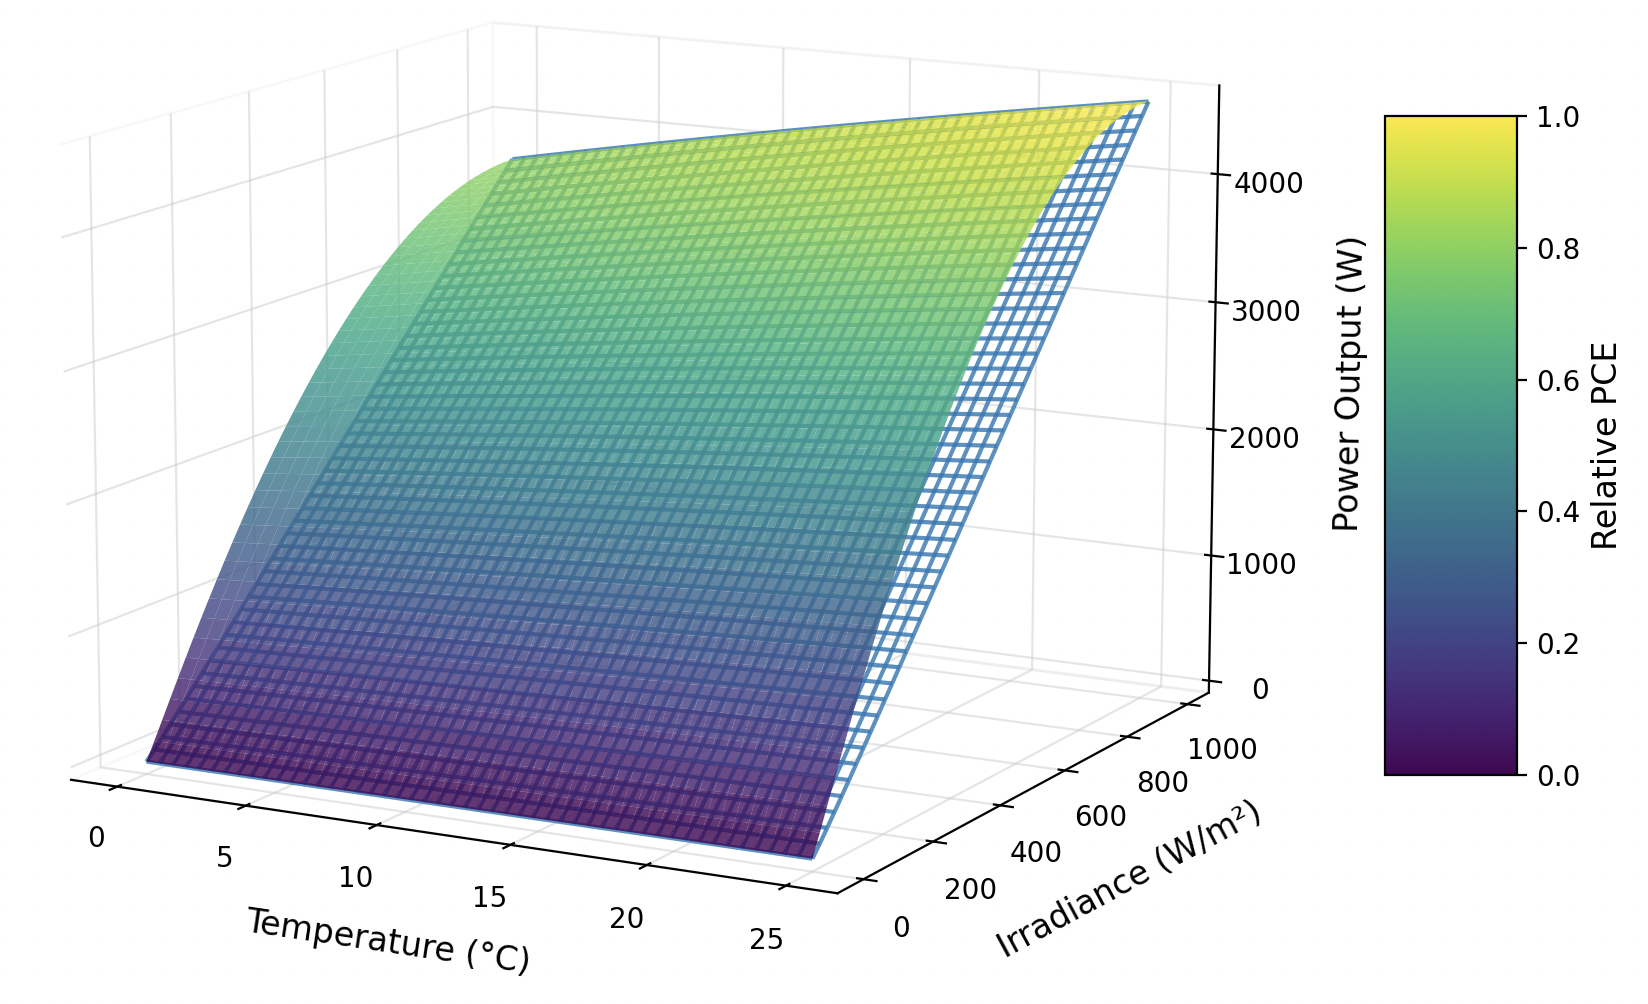
\includegraphics[width=\columnwidth]{Figures/3d_PV.png}
                \caption{Power generation from 1 to 2 \(\delta_{mat}\)}
            \end{figure}

        \item<only@2>[]
            \begin{figure}
                \centering
                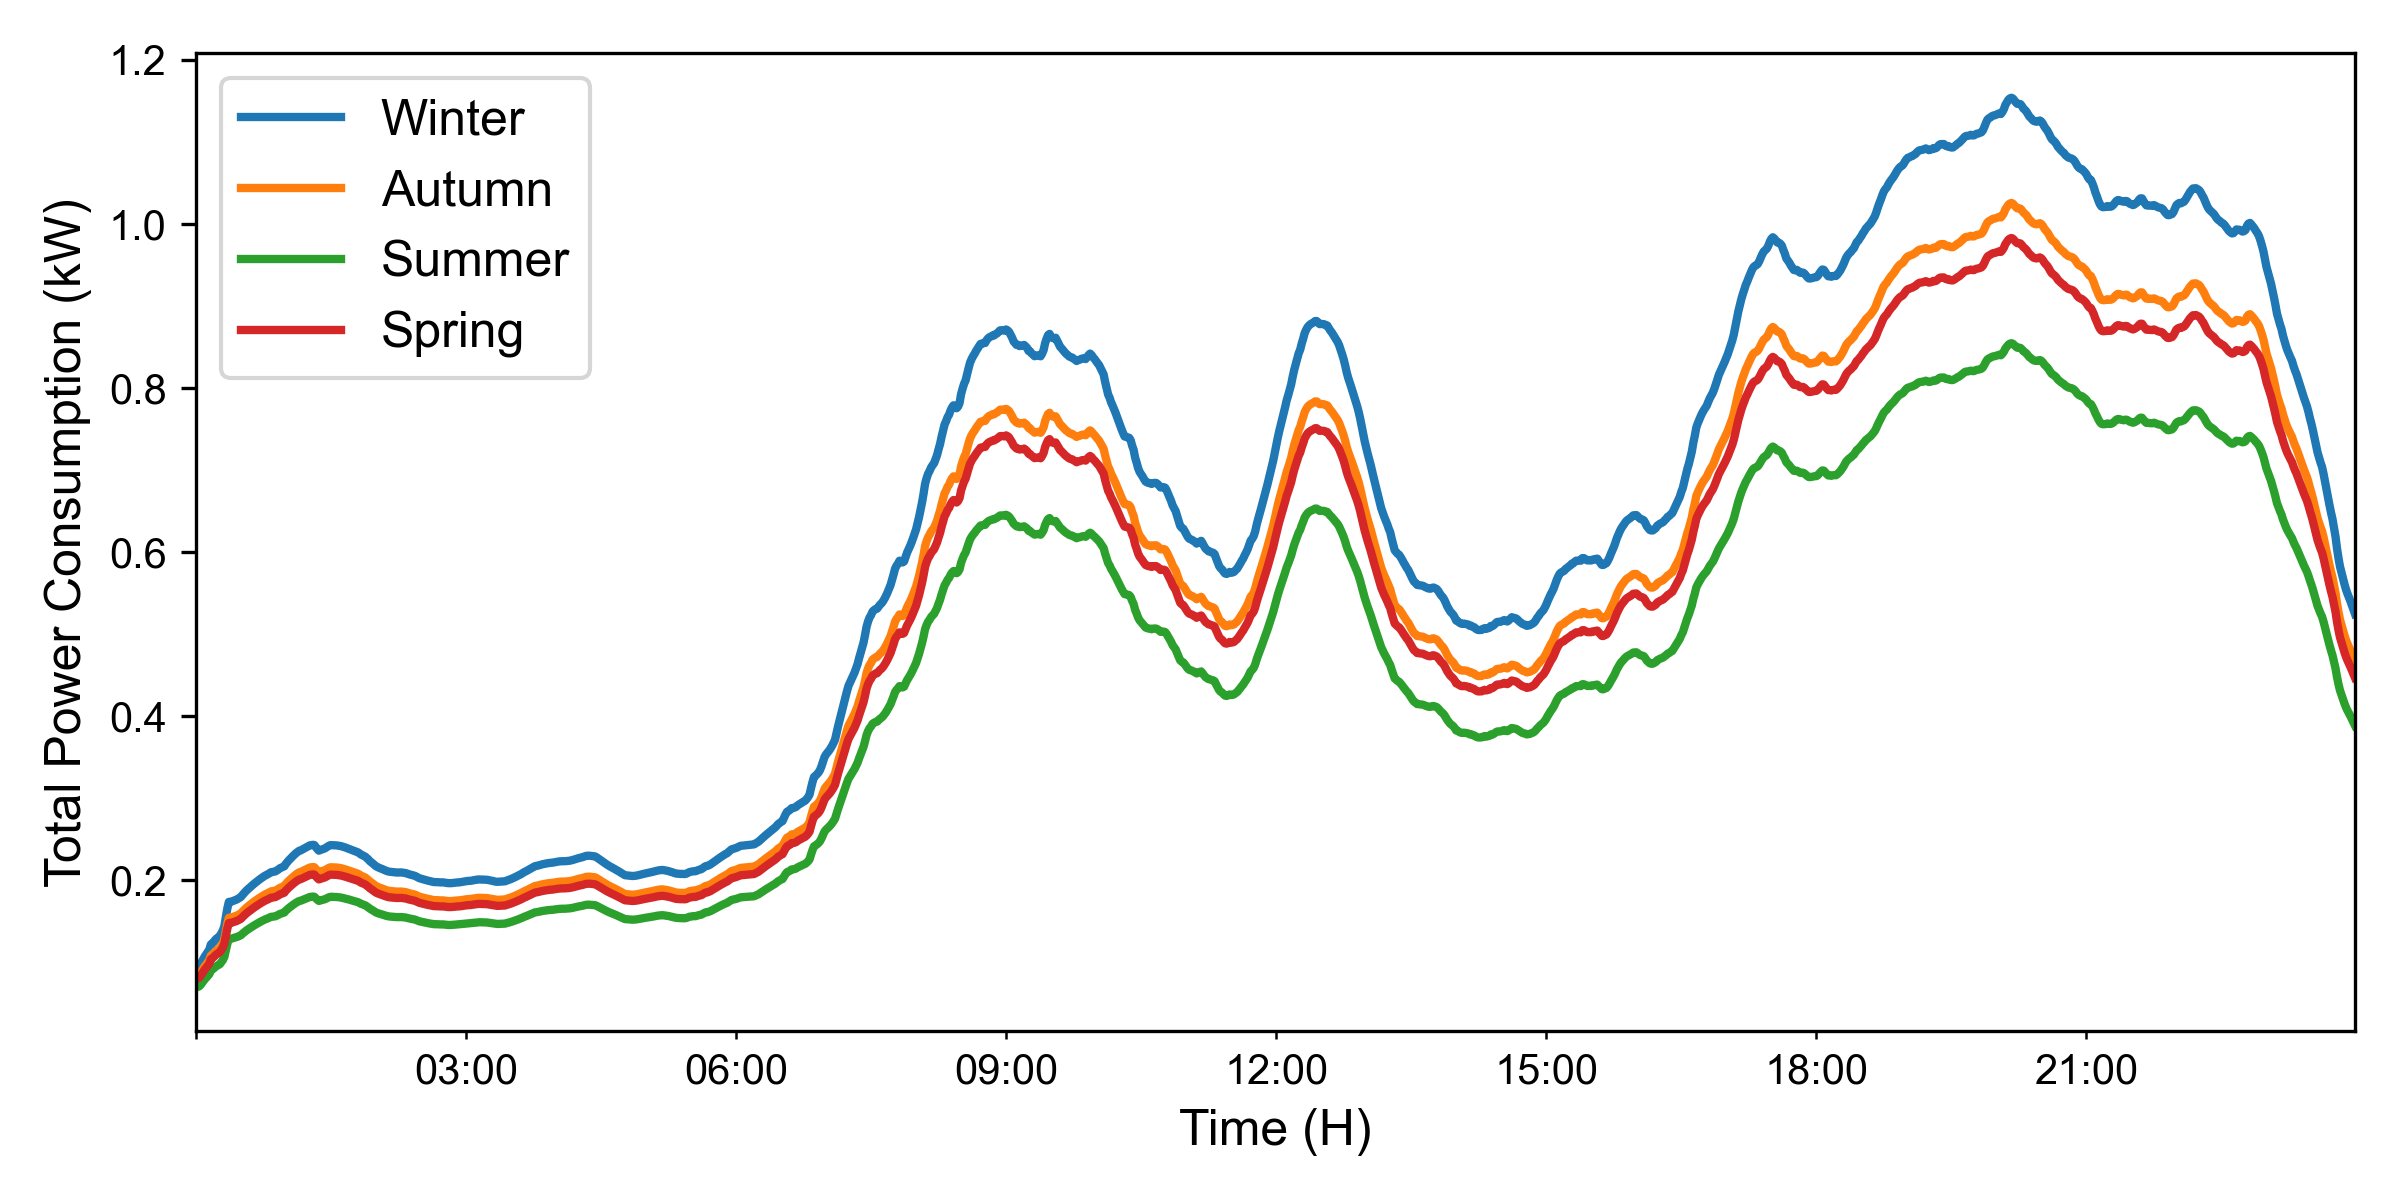
\includegraphics[width=\columnwidth]{Figures/load_season.png}
                \caption{Load utilised for calculating self-consumption accounting for season energy consumption increase}
            \end{figure}
            
        \item<only@3>[]
            \begin{figure}
                \centering
                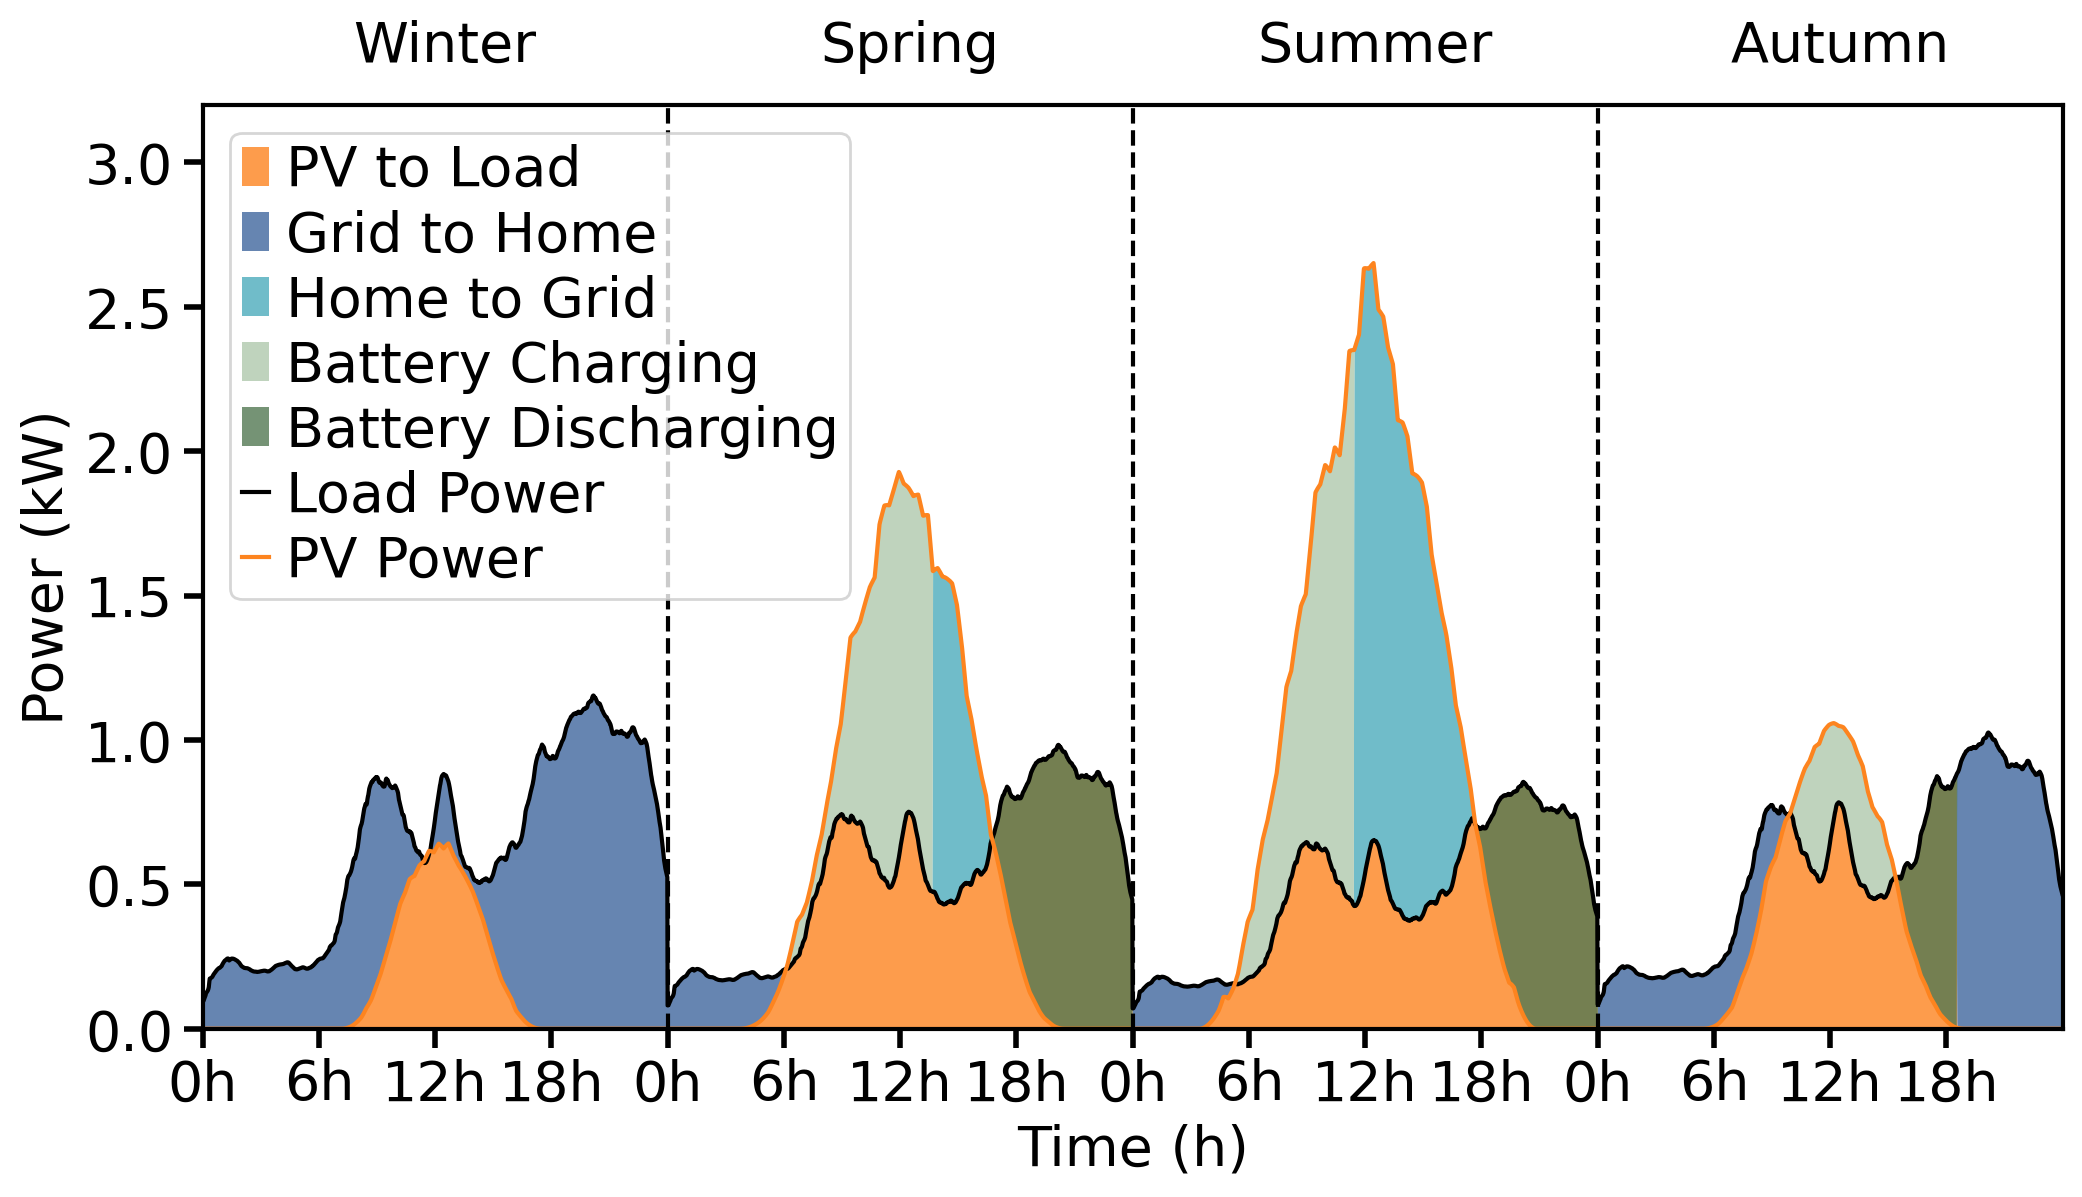
\includegraphics[width=\columnwidth]{Figures/SI_power_distribution.png}
                \caption{Power generation by Silicon technology per season}
            \end{figure}

        \item<only@4>[]
            \begin{figure}
                \centering
                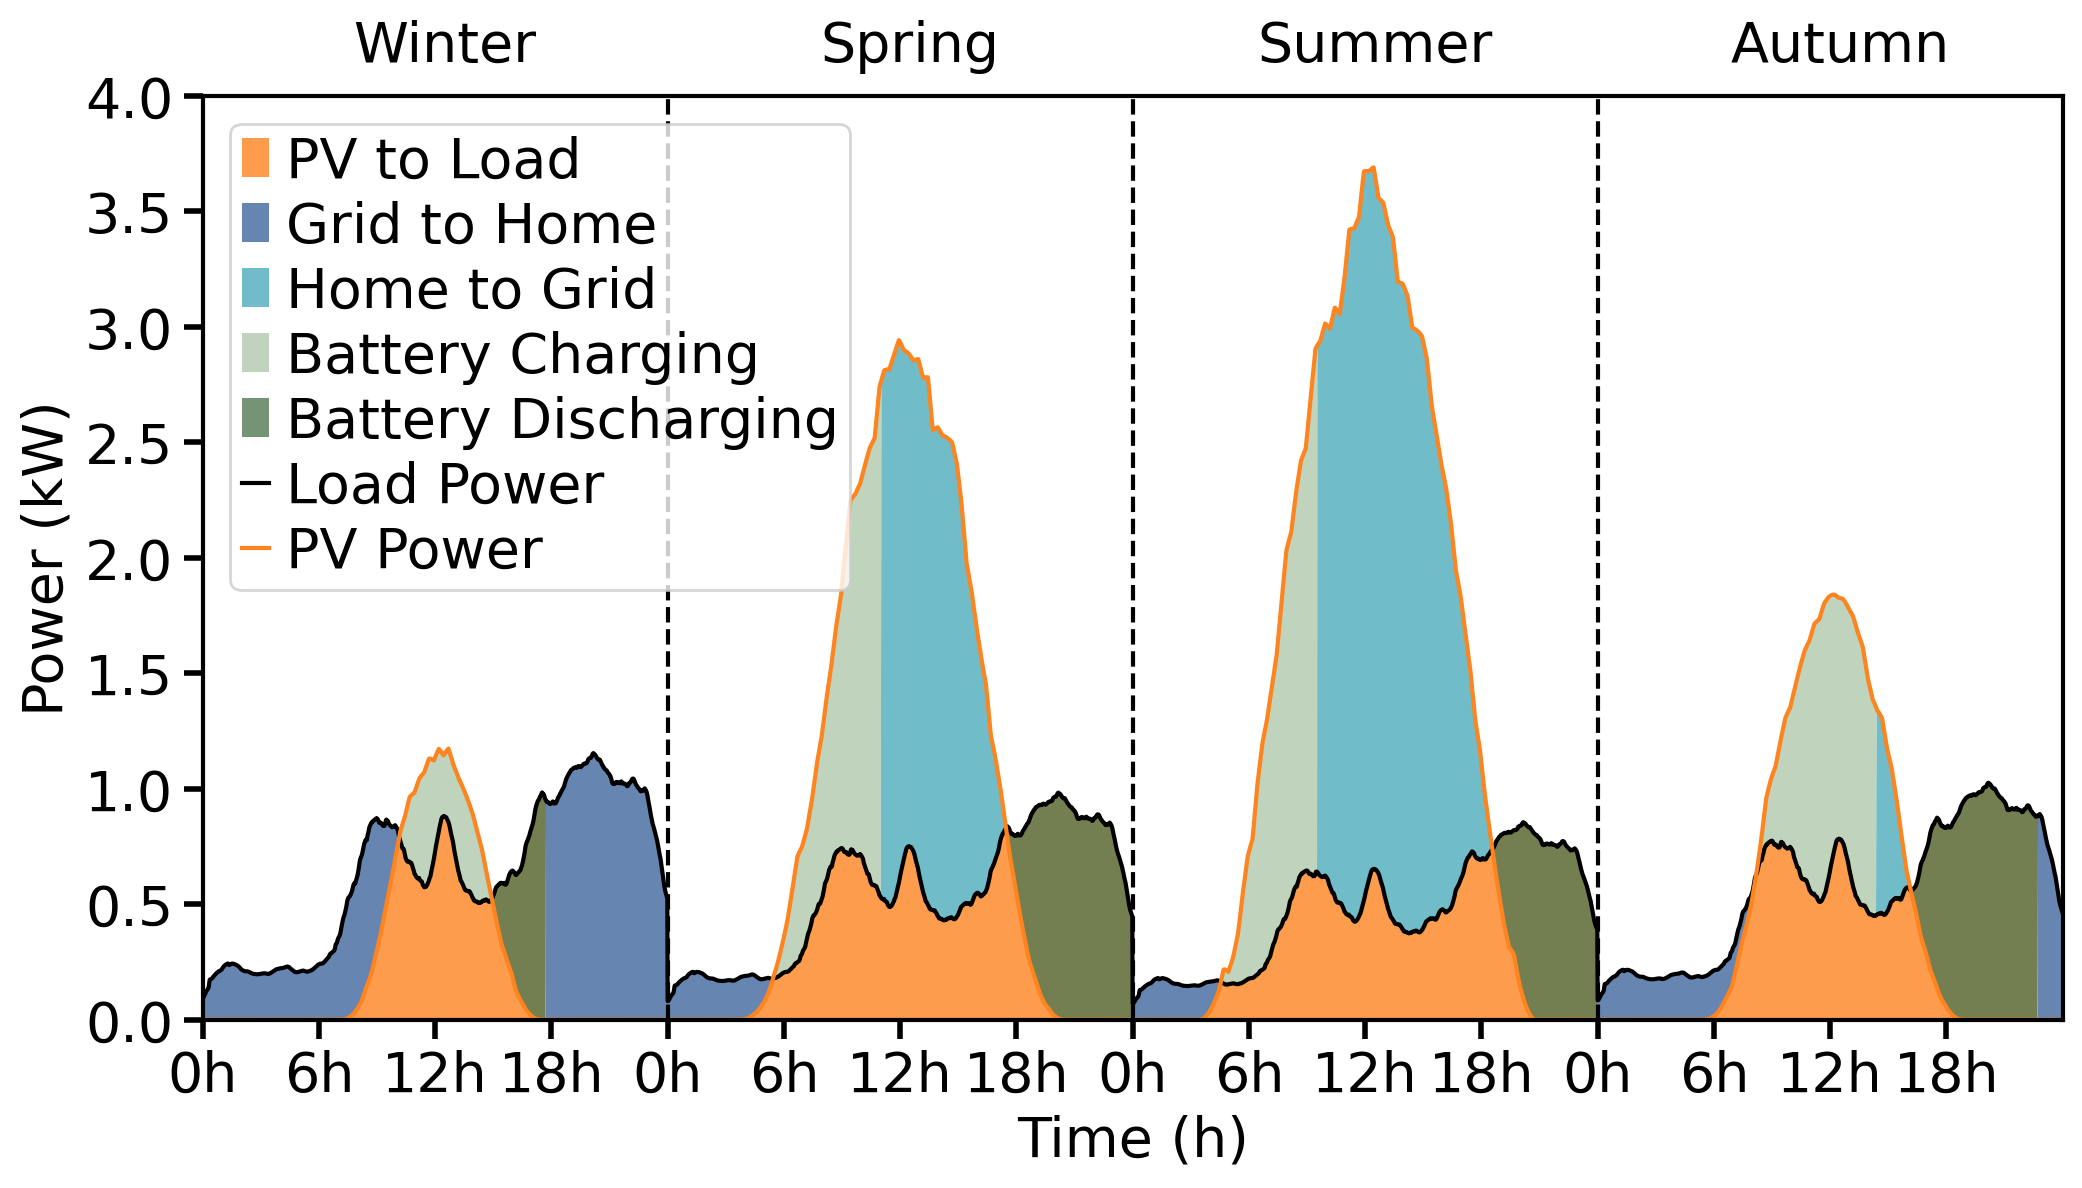
\includegraphics[width=\columnwidth]{Figures/LLE_power_distribution.png}
                \caption{Power generation by LLE technology per season}
            \end{figure}

        \item<only@5>[]
            \begin{figure}[htbp]
                \centering
                
                \begin{minipage}{0.24\linewidth}
                    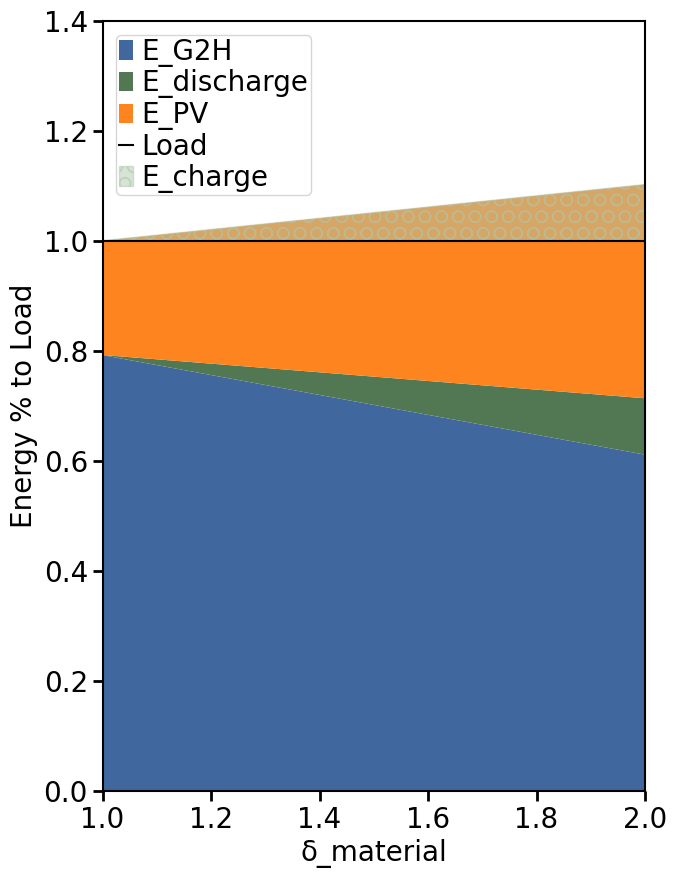
\includegraphics[width=\linewidth]{Figures/winter.png}
                    \caption{Winter}
                \end{minipage}\hfill%
                \begin{minipage}{0.24\linewidth}
                    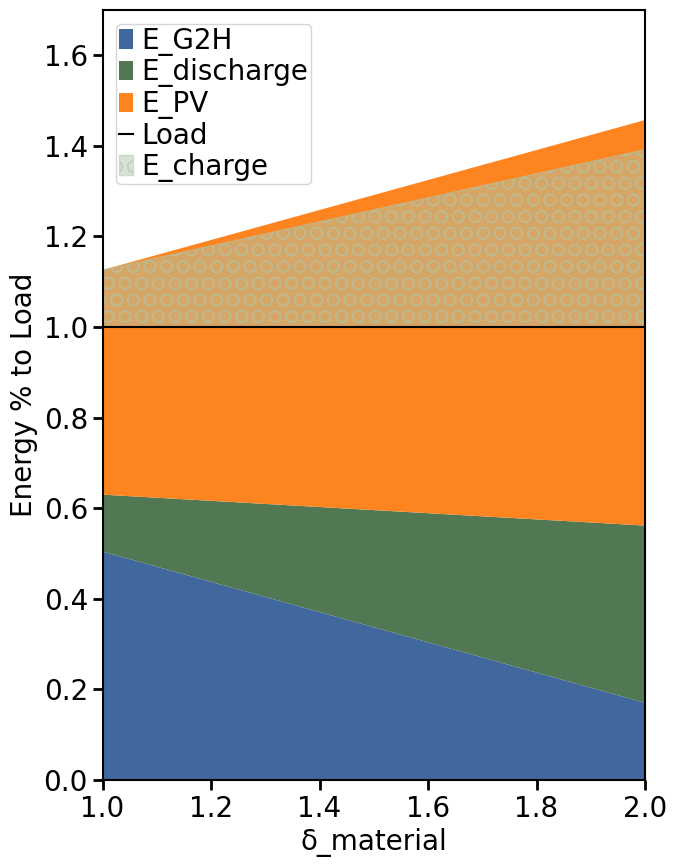
\includegraphics[width=\linewidth]{Figures/autumn.png}
                    \footnotesize
                    \caption{Autumn}
                \end{minipage}\hfill
                \begin{minipage}{0.24\linewidth}
                    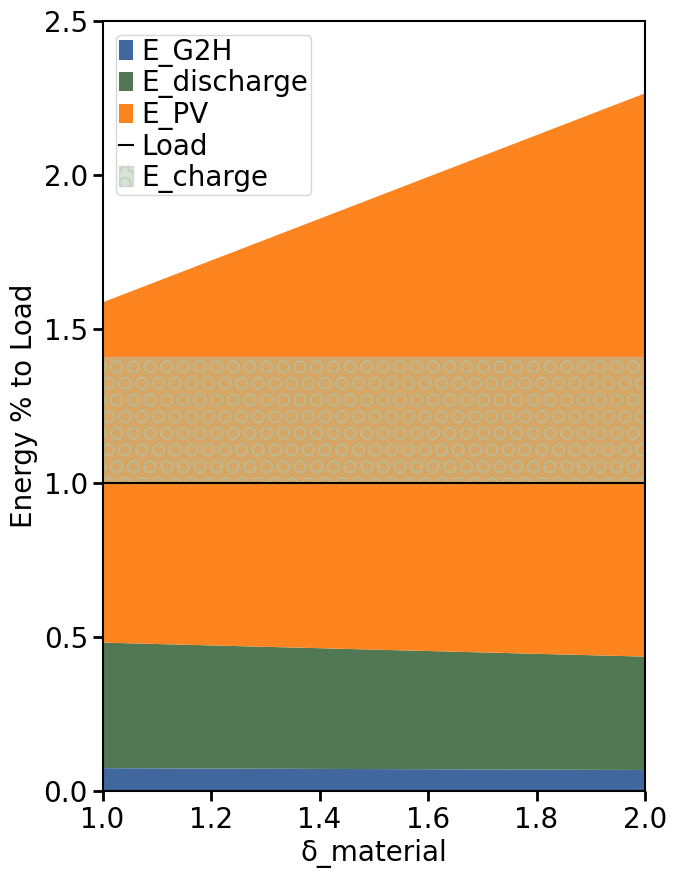
\includegraphics[width=\linewidth]{Figures/spring.png}
                    \footnotesize
                    \caption{Spring}
                \end{minipage}\hfill
                \begin{minipage}{0.24\linewidth}
                    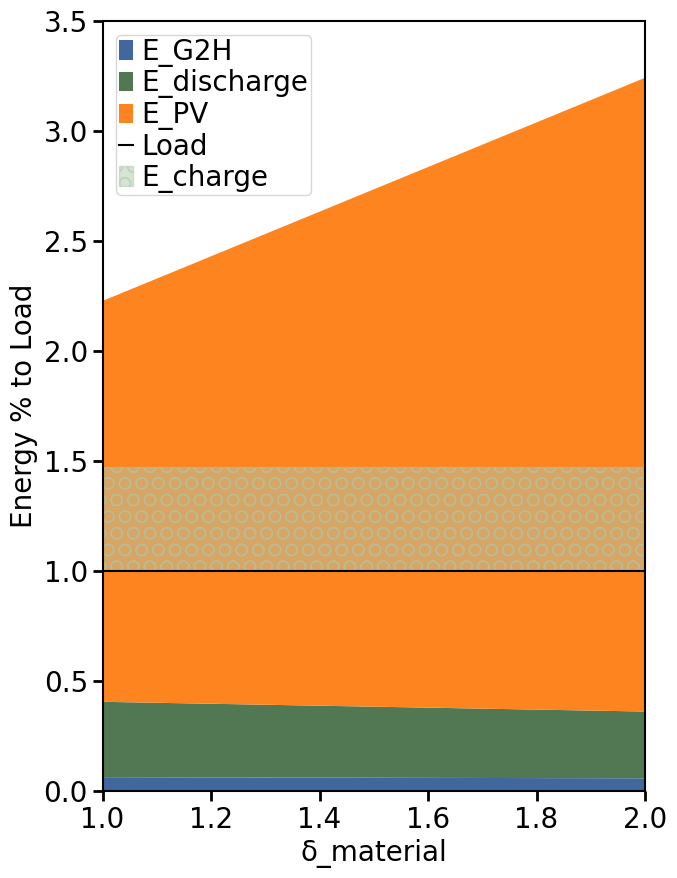
\includegraphics[width=\linewidth]{Figures/summer.png}
                    \footnotesize
                    \caption{Summer}
                \end{minipage}\hfill
            \end{figure} 

    \end{itemize}
    
\end{frame}



\section{}

\begin{frame}[c]{}
  \centering \Huge
  \emph{Thank you for your attention.}
\end{frame}

%%%%%%%%%%%%%%%%%%%%%%%%%%%%%%%%%%%%%%%%%%%%%%%%%%%%%%%%%%%%
% \section{References}
%% For showing numbered references
% \setbeamertemplate{bibliography item}{\insertbiblabel}

% \begin{frame}[allowframebreaks]{References}

    %% When some or all papers from the bib file are not cited
    % \nocite{*}  % for all entries in the used bib data file
    % \nocite{<key>} % for a single one

    % \bibliographystyle{ieeetr}
    % \bibliographystyle{apalike}
    % \footnotesize
    % \bibliography{References.bib}
%     \printbibliography

% \end{frame}
%%%%%%%%%%%%%%%%%%%%%%%%%%%%%%%%%%%%%%%%%%%%%%%%%%%%%%%%%%%%


\end{document}